We will propose an evolution of the basic case that reduces the search space and adds some robustness. The idea is that instead of swithcing strategies on and off based on the current short-term Sharpe-Ratio being above a certain threshold, we care about ranking the performance of strategies making the assumption that the best ones will still perform well. There are two reasons why this choice makes sense: first of all ranking removes the burden of optimizing some parameters reducing the risk of overfitting. Secondarily, ranking is a much more robust statistics than a simple threshold, we expect therefore that this method will perform better out of sample. We still have to apply a first filter as for the previous case (fixing the parameters as they have been chosen for method 1), then we will grid-search for an optimal window where strategies are ranked by Sharpe Ratio.\\
Notice that we also have to set a parameter that is the number of strategies that will be considered best ones after being ranked. The idea here is that this number is given by what the in-company execution system and the risk management framework can withstand, that is about 50 strategies at the same time. More precisely we will select the top 50 strategies (out of 13000!) but only if their Sharpe-Ratio is still positive in the last period.

\begin{center}
	\centering
    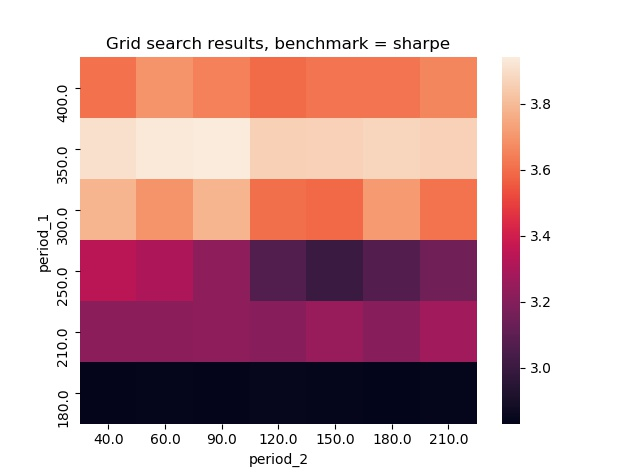
\includegraphics[width=0.6\textwidth]{GridSearches/Sharpe_Ranking/Figure_1.jpeg}
	\captionof{figure}{GridSearch for the two windows of the Sharpe Ratio}
	\label{Sharpe_Ranking_1}
\end{center}

\begin{center}
	\centering
	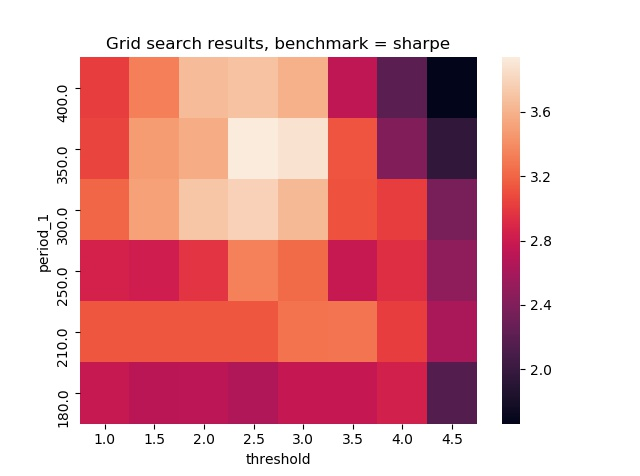
\includegraphics[width=0.6\textwidth]{GridSearches/Sharpe_Ranking/Figure_2.jpeg}
	\captionof{figure}{GridSearch for one window vs the threshold for the Sharpe Ratio}
	\label{Sharpe_Ranking_2}
\end{center}

\begin{center}
	\centering
	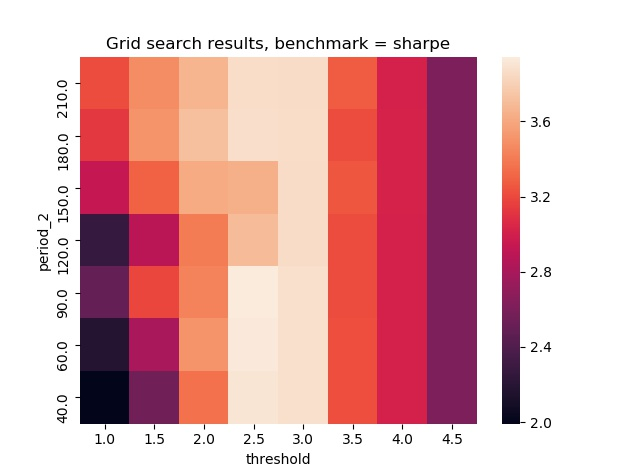
\includegraphics[width=0.6\textwidth]{GridSearches/Sharpe_Ranking/Figure_3.jpeg}
	\captionof{figure}{GridSearch for one window vs the threshold for the Sharpe Ratio}
	\label{Sharpe_Ranking_3}
\end{center}

As we can see the performance is on average much better, but also the results are more reliable. The in-sample gridsearch suggests that the optimal value for the filtering Sharpe is about 350 trading days, while for the threshold the ideal value seems to be in the 2.5/3 area. The length of the window for the Sharpe ratio used to rank doesn't seem to be extremely relevant but still it seems  to suggest that optimal values might be in the 90s.\\
Using these results we test the method in sample and obtain a nice equity line:

\begin{center}
	\centering
	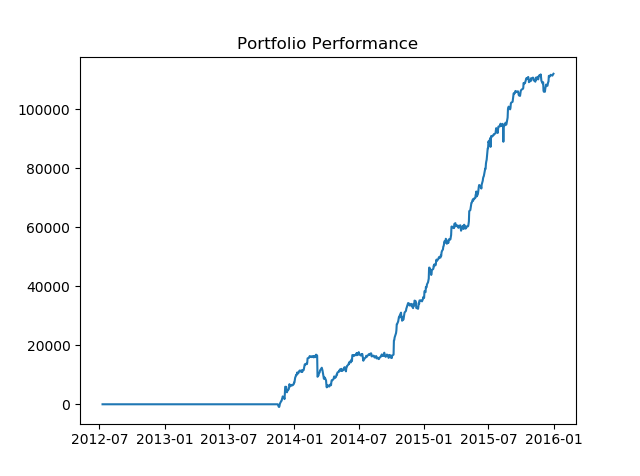
\includegraphics[width=0.6\textwidth]{GridSearches/Sharpe_Ranking/In_Sample_performance.png}
	\captionof{figure}{In-Sample performance for the Sharpe-ranking method}
	\label{Sharpe_Ranking_in_sample}
\end{center}

We can see that the statistics are quite good with an in-sample Sharpe-Ratio up to 3.69.

\begin{table}
	\centering
	\begin{tabular}{c|c}
		\textbf{Statistic} & \textbf{Value} \\\hline
		Sharpe Ratio & 3.696 \\ 
		Sortino Ratio & 4.2479 \\ 
		Omega Ratio & 2.13 \\ 
		Skewness & -0.6776 \\ 
		Kurtosis & 15.9628 \\ 
		Maximum Drawdown (\% duration/duration) & 14.4 \\ 
		Longest Drawdown (days) & 80.0 \\ 
		Winning Days & 63.3574 \\ 
	\end{tabular}
	\caption{\label{tab:widgets} Statistics for the in-sample performance of the Sharpe-Ranking method.}
\end{table}

